\documentclass[a4paper,french,bookmarks]{article}
\usepackage{./Structure/4PE18TEXTB}

\renewcommand{\thesection}{\Roman{section}} 
\begin{document}
\stylizeDoc{Physique}{Devoir Maison 6}{Accordeur de guitare}
\newboxans

\begin{minipage}{0.6\linewidth}
	On se propose d'étudier quelques aspects d'un accordeur de guitare.
	La guitare classique comporte six cordes : \textsl{mi} grave, \textsl{la}, \textsl{ré}, \textsl{sol}, \textsl{si}, \textsl{mi} aigu. 
	Les fréquences fondamentales théoriques de vibration de ces cordes, notées
	$f_\text{ac}$ sont données dans le tableau ci-contre.\\[-5pt]
	
	On souhaite accorder une corde légèrement désaccordée : on notera $f_\text{co}$ la fréquence fondamentale de
	vibration de la corde en question.
\end{minipage}
%
\hfill
%
\begin{minipage}{0.35\linewidth}
	\centering
	\begin{tabular}{c|c}
		Corde 				& Fréquence $f_\text{ac}$	\\ \hline\hline
		\textsl{mi} grave 	& \SI{82,4}{\hertz} 		\\
		\textsl{la} 		& \SI{110,0}{\hertz} 		\\
		\textsl{ré} 		& \SI{146,8}{\hertz} 		\\
		\textsl{sol} 		& \SI{196}{\hertz} 			\\
		\textsl{si} 		& \SI{246,9}{\hertz} 		\\
		\textsl{mi} aigu 	& \SI{329,6}{\hertz} 		\\
	\end{tabular}
\end{minipage}

\strong{Principe de l'accordeur :}
%
\begin{enumerate}
	\itt Sélection de la corde à accorder (donc $f_\text{ac}$ est fixée).
	
	\itt Création d'un signal carré de référence de fréquence $f_\text{ac}$.
	
	\itt Enregistrement du signal $u_\text{e}(t)$ provenant de l'excitation de
	la corde à accorder : signal quelconque, d'amplitude assez faible,
	de fréquence $f_\text{co}$.
	
	\itt Amplification et filtrage de ce signal.
	
	\itt Extraction de la fondamentale du signal : obtention d'un signal
	sinusoïdal de fréquence $f_\text{co}$ par l'utilisation d'un filtre à
	fréquence caractéristique réglable par le signal extérieur de
	référence.
	
	\itt Mise en forme de ce signal : obtention d'un signal carré de
	fréquence $f_\text{co}$.
	
	\itt On a donc à disposition deux signaux carrés (signaux logiques)
	de fréquences respectives $f_\text{ac}$ et $f_\text{co}$. Dans les accordeurs
	récents le traitement est numérique : les signaux sont envoyés dans un
	calculateur numérique intégré qui calcule l'écart de fréquence et
	indique à l'utilisateur quand la corde est accordée, c'est-à-dire
	quand $f_\text{co}=f_\text{ac}$.
\end{enumerate}

Ce principe général est schématisé ci-dessous :

\begin{center}
	\begin{tikzpicture}[elem/.style={minimum width=20mm, minimum height=15mm, align=center}]
		\node (choix) [elem, text width=30mm] {Choix de la corde (donc de la fréquence)} ;
		\node (oscil) [elem, draw, right=10mm of choix] {Oscillateur} ;
		\draw [-Latex] (choix) -- (oscil) ;
		\node (utn) [elem, draw, right=40mm of oscil, text width=30mm] {Unité de traitement numérique} ;
		\draw [-Latex] (oscil) -- (utn) coordinate [midway] (fac) node [midway, above] {Signal carré à $f_\text{ac}$} ;
		\node (compa) [elem, draw, below=15mm of utn] {Comparateur} ;
		\draw [-Latex] (compa) -- (utn) node [midway, left,text width=20mm,align=center] {Signal carré à $f_\text{co}$} ;
		\node (Fc) at (fac |- compa) [elem, draw, text width=20mm] {Filtre commandé $F_\text{c}$} ;
		\draw [-Latex] (Fc) -- (compa) node [midway, above] {$u_3$} ;
		\draw [-Latex] (fac) -- (Fc) node [midway, left] {$u_{\rm ref}$} ;
		\node (Fb) [elem, draw, text width=20mm, left=15mm of Fc] {Amplification sélective $F_\text{b}$} ;
		\draw [-Latex] (Fb) -- (Fc) node [midway, above] {$u_2$} ;
		\node (Fa) [elem, draw, text width=20mm, left=15mm of Fb] {Passe-haut $F_\text{a}$} ;
		\draw [-Latex] (Fa) -- (Fb) node [midway, above] {$u_1$} ;
		\node (fco) [elem, text width=20mm, left=15mm of Fa] {Signal corde à $f_\text{co}$} ;
		\draw [-Latex] (fco) -- (Fa) node [midway, above] {$u_\text{e}$} ;
	\end{tikzpicture}
\end{center}

On s’intéresse au traitement du signal venant de la corde. 
Nous allons nous limiter à l'étude des filtres $F_\text{a}$, $F_\text{b}$
et $F_\text{c}$.


\section{Le signal}

La figure \ref{signal} montre un exemple de signal électrique à
la sortie du micro d'une guitare électrique.

\begin{figure}
	\centering
	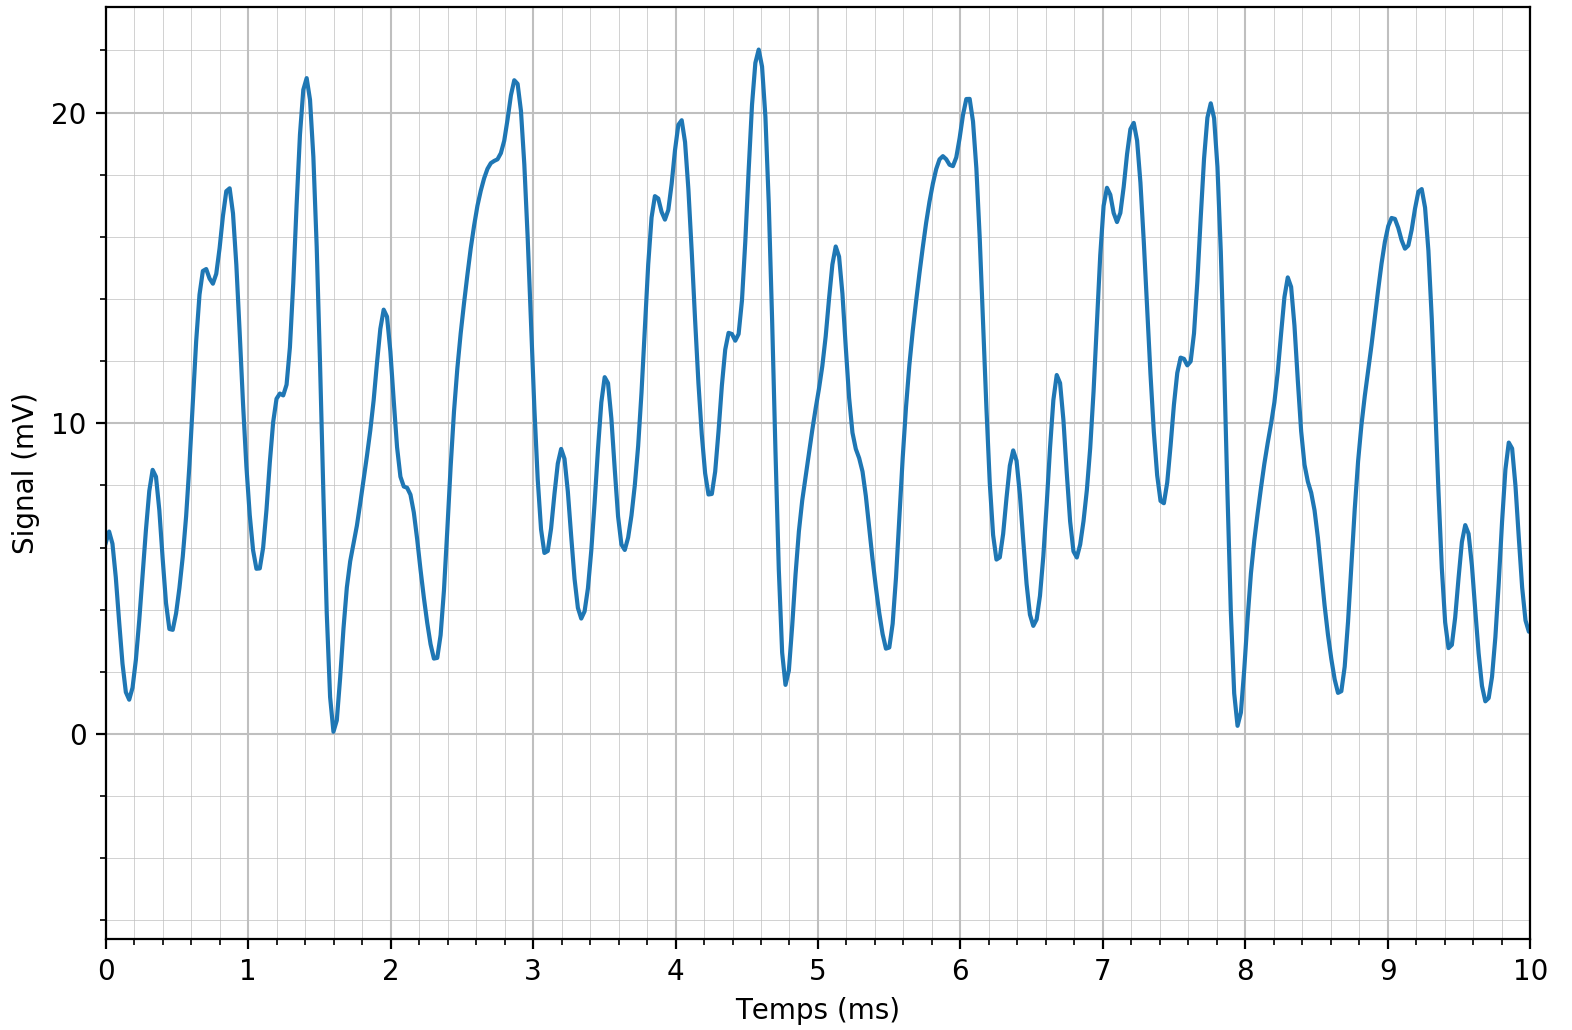
\includegraphics[scale=0.7]{dm6fig/fig_signal.png}
	\caption{Signal temporel issu de l'enregistrement du son de la guitare.}
	\label{signal}
\end{figure}   

\begin{enumerate}
    \item\label{qu:1} Donner une valeur approchée de la valeur moyenne de ce signal.
    
    \boxans{
        On trouve pour la moyenne de ce signal l'approximation suivante : \boxsol{$\phyavg{u_e} \approx \SI{10}{\mV}$}.
    }

    \item Donner une estimation de la valeur de la fréquence de ce signal (on peut supposer qu'en première approximation le signal est périodique).
    
    \boxans{
        Le motif entre \SI{1.1}{\ms} et $t_1 = \SI{1.6}{\ms}$ semble se répéter assez distinctement entre \SI{4.2}{\ms} et \SI{4.8}{ms}, puis entre \SI{7.4}{ms} et $t_2 = \SI{7.9}{ms}$, les variations en intensité pouvant s'expliquer par les conditions réelles de capture du signal par le micro de la guitare (bruit, mouvement, \dots).\\[-5pt]
        
        Ce motif fournit par ailleurs un point où la variation change brusquement pratique pour l'identification, notamment visible à $t_1$ et $t_2$. On a donc deux fois la période $T_\text{co}$ entre $t_1$ et $t_2$, d'où $T_\text{co} = \sfrac{1}{2}(t_2 - t_1)$.
        
        On a $f_\text{co} = \dfrac{1}{T_\text{co}}$ d'où \boxsol{$f_\text{co} = \dfrac{2}{t_2 - t_1}$}. L'application numérique donne \boxsol{$f_\text{co} = \SI{3.2e2}{\hertz}$}.
    }

    \item\label{qu:3} De quelle corde de guitare s'agit-il ?
    
    \boxans{
        On a $f_\text{co} \approx \SI{320}\hertz$, ce qui est proche du \boxsol{\textsl{mi} aigu}.
    }

    \item L'analyse spectrale de ce signal fera-t-elle apparaître des harmoniques ? Justifier.
    
    \boxans{
        En conditions réelles comme c'est ici le cas, la corde d'un instrument ne va pas qu'entrer en résonne seulement selon la fréquence fondamentale, mais selon une multitude de modes de vibrations qui lui sont possibles, correspondant aux harmoniques visibles dans une analyse spectrale.\\[-5pt]
        
        On voit par ailleurs sur la figure \ref{signal} que le signal est plus complexe qu'une simple sinusoïde, preuve qu'il est composé de plusieurs harmoniques. \boxsol{L'analyse spectrale de ce signal fera donc apparaître des harmoniques}.
    }

\end{enumerate}


\section{Premier filtre}

Avant toute chose, le signal électrique provenant du micro de la
guitare est envoyé sur le filtre $F_\text{a}$ ci-dessous.


\begin{center}
	\begin{tikzpicture}
		\draw(0,2) to[C,l_=$C_1$] (4,2) to[R,l_=$R_1$,v^<={$u_1$}] (4,0) node[cground,scale=0.8] {} ;
		\draw (0,0) node[cground,scale=0.8] {} to[open,v^>={$u_\text{e}$}] (0,2) ;
	\end{tikzpicture}
\end{center}


\begin{enumerate}[resume]
    \item En supposant l'entrée sinusoïdale, définir et exprimer la fonction de transfert $\underline{H}_1(\jj\omega)$ de ce filtre en fonction de $R_1$, $C_1$ et de la pulsation $\omega$ du signal.
    
    \boxans{
        En se plaçant en régime sinusoïdal forcé, on peut exprimer $u_1$ sous la forme $u_1(t) = U_\text{m}\cos(\omega t + \phi)$. On se donne alors les notations complexes $\underline{u}_1(t) = U_\text{m}e^{\jj(\omega t + \phi)} = \underline{U}_\text{m}e^{\jj\omega t}$ et $\underline u_\text{e} = e^{\jj\omega t}$.\\[-5pt]
        
        Par définition, on a $\underline H_1(\jj\omega) = \dfrac{\underline{u}_1}{\underline u_\text{e}} = \underline{U}_\text{m}$. On repère un pont diviseur de tension, on obtient donc $\underline u_1 = \dfrac{R_1}{R_1 + \frac{1}{\jj\omega C_1}}\underline u_\text{e}$. En multipliant finalement par $\jj\omega C$, on a donc \boxsol{$\underline H_1(\jj\omega) = \dfrac{R_1C_1\jj\omega}{1 + R_1C_1\jj\omega}$}.
    }

    \item De quel type de filtre s'agit-il ? Faire apparaître une pulsation caractéristique $\omega_1$ en fonction de $R_1$ et $C_1$ et préciser sa signification.
    
    \boxans{
        On remarque que $[R_1C_1] = T$, on  pose donc la pulsation caractéristique \boxsol{$\omega_1 = \dfrac{1}{R_1C_1}$}. Puisqu'on a un filtre $RC$ série du premier ordre, cette pulsation est aussi la \boxsol{pulsation de coupure}. On peut aussi poser la pulsation réduite $x = \dfrac{\omega}{\omega_1}$, donc $\underline H_1(x) = \dfrac{\jj x}{1 + \jj x}$. On a alors le gain :
        
        \[G_1(x) = \mod{\underline H_1(x)} = \dfrac{\mod{\jj x}}{1+\jj x} = \dfrac{x}{\sqrt{1+x^2}}\]
        
        Ainsi, on a $G_1(x) \lima{x \to 0} 0$ et $G_1(x) \lima{x \to +\infty} 1$. On a donc un \boxsol{filtre passe-haut du premier ordre}.
        
        On retrouve ce résultat sans le calcul par les circuits équivalents :\\
    
        \begin{minipage}[t]{0.45\textwidth}
            \strong{Circuit équivalent à très haute fréquence}
            
            \begin{center}
	            \begin{tikzpicture}
		            \draw(0,2) to (4,2) to[R,l_=$R_1$,v^<={$u_1 = u_\text{e}$}] (4,0) node[cground,scale=0.8] {} ;
		            \draw (0,0) node[cground,scale=0.8] {} to[open,v^>={$u_\text{e}$}] (0,2) ;
	            \end{tikzpicture}
            \end{center}
        \end{minipage}
        %
        \hfill\vline\hfill
        %
        \begin{minipage}[t]{0.45\textwidth}
            \strong{Circuit équivalent à très basse fréquence}
            
            \begin{center}
	            \begin{tikzpicture}
		            \draw(0,2) to[nos] (4,2) to[R,l_=$R_1$,v^<={$u_1 = 0$}] (4,0) node[cground,scale=0.8] {} ;
		            \draw (0,0) node[cground,scale=0.8] {} to[open,v^>={$u_\text{e}$}] (0,2) ;
	            \end{tikzpicture}
            \end{center}
        \end{minipage}
    }

    \item Tracer sans calcul l'allure du diagramme de Bode asymptotique relatif au gain en décibels.
    
    \boxans{
        Puisque l'on a un filtre passe-haut d'ordre 1, $G_\text{dB}$ à l'échelle logarithmique a une asymptote horizontale lorsque $x$ tend vers $+\infty$ et une asymptote d'équation $y = 20x$ lorsque $x$ tend vers $-\infty$. Elle passe également par $\SI{-3}{\dB}$ en $x = 1$.
        
        \begin{center}
            \boxsol{
            \pgfplotsset{width=10cm, height=8cm}
            \begin{tikzpicture}
                \begin{axis}[
                    axis lines = left,
                    xlabel=$\mathsf{x}$,
                    ylabel=$\mathsf{G}_\textsf{dB} \ \textsf{(dB)}$,
                    domain=0.08:12,
                    xmode=log,
                    log basis x={10},
                    xmin=0.08,
                    xmax=12,
                    ymin=-22,
                    ymax=2,
                    ytick={-20, -10, -3, 0},
                    log ticks with fixed point,
                    xticklabel={$\mathsf{10^{\pgfmathprintnumber{\tick}}}$},
                    yticklabel={$\mathsf{\pgfmathprintnumber{\tick}}$},
                    font=\footnotesize,
                    grid = both,
                    grid style = {line width = .1pt, draw = gray!30},
                    major grid style = {line width=.2pt,draw=gray!50},
                ]
                    \addplot[color=main3, line width=0.3mm, domain=0.08:1] {20*ln(x)/ln(10)};
                    \addplot[color=main3, line width=0.3mm, domain=1:12] {0*x};
                    \addplot[color=main1, dashed, line width=0.6mm] {20*ln(x/sqrt(1+x^2))/ln(10)};
                    \addplot[mark=+,main7, mark size=2mm, line width=1mm, thick] coordinates {(1,-3)};
                \end{axis}
            \end{tikzpicture}
            }
        \end{center}
    }

    \item\label{qu:8} On a choisi $R_1 = \SI{100}{\kilo\ohm}$ et $C_1 = \SI{100}{\nano\farad}$. Déterminer et calculer la fréquence de coupure $f_1$ à \SI{-3}{\deci\bel} de ce filtre. Au vu de l'allure du signal de la figure \ref{signal}, quel est le rôle de ce premier filtre ?
    
    \boxans{
        On a la pulsation de coupure $\omega_\text{c} = 2\pi f_1$. Or $\omega_\text{c} = \omega_1 = \dfrac{1}{R_1C_1}$, donc \boxsol{$f_1 = \dfrac{1}{2\pi R_1C_1}$}. L'application numérique donne \boxsol{$f_1 = \SI{15,9}{\hertz}$}.\\[-5pt]
        
        Le filtre ne va donc que marginalement affecter la partie du signal que l'on souhaite étudier, à savoir le son de la note fondamentale jouée par la corde désaccordée. Le rôle de ce filtre est donc d'éliminer les potentiels sons parasites capturés par le micro de basse fréquence (bruit sourd causé par un choc du micro contre son support lors du mouvement de la guitare, bruit, \dots). Il filtrera par ailleurs \guill{l'harmonique de fréquence nulle}, qui correspond à la valeur moyenne du signal $\phyavg{u_e}$.
    }

\end{enumerate}

\section{Deuxième filtre}

Dans cette sous-partie, les signaux sont sinusoïdaux et on utilise un composant appelé \textit{amplificateur linéaire intégré} (ALI). 
Dans la suite, on note $V_M$ le potentiel en un point M (et $\underline{V}_M$ le potentiel complexe associé). 

\subsection{Préambule}

\begin{minipage}{0.5\linewidth}
	On admet qu'un ALI vérifie les propriétés suivantes :
	\begin{itemize}
		\item $i_+=i_-=0$ et $i_S$ est inconnu.
		\item $u=V_A-V_B=0$.
	\end{itemize}
\end{minipage}
%
\hspace{2cm}
%
\begin{minipage}{0.3\linewidth}
	\begin{tikzpicture}
		\node[en amp,yscale=0.8,noinv input up](opamp){} ;
		\draw (opamp.+) to[short,i_<=$i_+$,-*] ++(-1,0) coordinate (A) node[above] {A} ;
		\draw (opamp.-) to[short,i<=$i_-$,-*] ++(-1,0) coordinate (B) node[below] {B} ;
		\draw (opamp.out) to[short,i=$i_S$] ++(1,0) ;
		\draw ($(A)+(-0.3,0)$) to[open,v<={$u$}] ($(B)+(-0.3,0)$) ; 
	\end{tikzpicture}
\end{minipage}
\hfill\newline

On considère le filtre ci-dessous. La position de la masse nous indique que la tension d'entrée est $e=V_A$ et que la tension de sortie est $s=V_S$.

\begin{center}
	\begin{tikzpicture}[yscale=0.7]
		\node[en amp,yscale=0.8,noinv input up] (opamp) {} ;
		\draw (opamp.-) to[short,i_<=$i_-$] ++(0,-1.6) coordinate (B) node[above left] {$B$} ;
		\draw (opamp.out) node[above] {$S$} to[short,*-] (opamp.out|-B) to[R,l={$\underline{Z}'$},-*] (B) 
			to[R,l_={$\underline{Z}$}] ++(0,-2) coordinate (G) node[cground] {}
		;
		\draw (opamp.+) to[short,i_<=$i_+$,-*] ++ (-2,0) node[left] {$A$} coordinate (A) ;
		\draw (A) to[open,v<={$e$}] (A|-G) node[cground] {} ;
		\draw (opamp.out) --++ (2,0) coordinate (S') to[open,v^<={$s$}] (S'|-G) node[cground] {} ;
	\end{tikzpicture}
\end{center}
\hfill

\begin{enumerate}[resume]
	\item A l'aide de la loi des mailles en B, démontrer que :
	
	\begin{equation}
		\dfrac{\underline{V}_B}{\underline{Z}}=\dfrac{\underline{V}_S - \underline{V}_B}{\underline{Z'}}	
	\end{equation}
	
	\boxans{
	    On pose $\underline i_Z$, $\underline i_{Z'}$, $\underline u_Z$ et $\underline u_{Z'}$ les intensités et tensions complexes au niveau de $\underline Z$ et de $Z'$. Par loi des noeuds, on a $\underline i_Z = \underline i_- + \underline i_{Z'}$. Or $\underline i_- = 0$ donc $\underline i_Z = \underline i_{Z'}$. Ainsi $\dfrac{\underline u_Z}{\underline Z} = \dfrac{\underline u_{Z'}}{\underline{Z'}}$.
	    
	    On oriente par cohérence $\underline u_Z$ et $\underline u_{Z'}$ selon une même convention. On a donc $k = \pm 1$ tel que :
	    
	    \[ \underline u_Z = k\underline V_B \qquad\et\qquad \underline u_{Z'} = k\left(\underline V_S - \underline V_B\right)\]
	    
	    On en déduit $\dfrac{k\underline{V}_B}{\underline{Z}} = \dfrac{k\left(\underline{V}_S - \underline{V}_B\right)}{\underline{Z'}}$ donc \boxsol{$\dfrac{\underline{V}_B}{\underline{Z}}=\dfrac{\underline{V}_S - \underline{V}_B}{\underline{Z'}}$}.
	}

	\item\label{qu:10} Exprimer la fonction de transfert $\underline{H}$ en fonction de $\underline{Z}$ et $\underline{Z}'$.
	
	\boxans{
	    On a $\underline H = \dfrac{\underline s}{\underline e} = \dfrac{\underline V_S}{\underline V_A}$. Or $\underline V_A - \underline V_B = 0$ donc $\underline V_A = \underline V_B$ d'où $\underline H = \dfrac{\underline V_S}{\underline V_B}$. Or d'après le résultat précédent :\\[-5pt]
	    
	    \[ \dfrac{\underline{V}_S - \underline{V}_B}{\underline{Z'}} = \dfrac{\underline{V}_B}{\underline{Z}} \qquad \text{donc} \qquad \dfrac{\underline V_S}{\underline{Z'}} = \underline V_B\left(\dfrac{1}{\underline Z} + \dfrac{1}{\underline Z'}\right) \qquad \text{donc} \qquad \dfrac{\underline V_S}{\underline V_B} = \underline{Z'}\left(\dfrac{1}{\underline Z} + \dfrac{1}{\underline Z'}\right)\]
	    
	    Donc \boxsol{$\underline H = 1 + \dfrac{\underline{Z'}}{\underline Z}$}.
	}
	
	\item Que devient $\underline{H}$ si $\underline{Z}$ et $\underline{Z'}$ sont des résistances ($\underline{Z}=R$ et $\underline{Z'}=R'$) ? Justifier que le montage est bien un amplificateur.
	
	\boxans{
	    On a alors $\underline H$ constant et réel $H = 1 + \dfrac{R'}{R}$. Or on a \boxsol{$s(t) = He(t)$}, de plus $R' > 0$ et $R > 0$ donc $\dfrac{R'}{R} > 0$.\\[-5pt]
	    
	    On en déduit que $H > 1$, ce qui justifie le \boxsol{comportement amplificateur}.
	}
\end{enumerate}

\subsection{Amplification (légèrement) sélective}

En sortie du filtre $F_\text{a}$ le signal $u_1(t)$ est envoyé sur le filtre $F_\text{b}$ ci-dessous.

\begin{center}
	\begin{tikzpicture}[yscale=0.7]
		\node[en amp,yscale=0.8,noinv input up] (opamp) {} ;
		\draw (opamp.-) --++ (0,-3.5) coordinate (B) ;
		\draw (opamp.out) node[above] {$S$} to[short,*-] (opamp.out|-B) to[R,l={$R_2$},-*] (B) 
			to[R,l_={$R_3$}] ++(0,-2) coordinate (G) node[cground] {}
		;
		\draw (opamp.+) to[short,-*] ++ (-2,0) node[left] {$A$} coordinate (A) ;
		\draw (A) to[open,v<={$u_1$}] (A|-G) node[cground] {} ;
		\draw (opamp.out) --++ (2,0) coordinate (S') to[open,v^<={$u_2$}] (S'|-G) node[cground] {} ;
		\draw ($(B)+(0,1.2)$) coordinate (B') to[C,l={$C_2$},*-*] (B'-|opamp.out) ; 
	\end{tikzpicture}
\end{center}

\begin{enumerate}[resume]
	\item Quelle est l'impédance $\underline{Z}_\text{eq}$ de la branche constituée par $R_2$ en parallèle avec $C_2$ ?
	
	\boxans{
	    L'admittance de la branche constituée par $C_2$ est $\jj \omega C_2$ et celle de la branche constituée par $R_2$ est $\dfrac{1}{R_2}$. L'impédance des deux branches en parallèles vaut l'inverse de la somme des admittances, soit :
	    
	    \[ \underline{Z}_\text{eq} = \dfrac{1}{\jj\omega C_2 + \frac{1}{R_2}} \qquad\text{donc}\qquad \boxsol{$\underline{Z}_\text{eq} = \dfrac{R_2}{1 + R_2C_2\jj \omega}$}\]
	}

	\item Déduire de la question \enumref{qu:10} l'expression de la fonction de transfert $\underline{H}_2$ de ce filtre en fonction de $R_2$, $R_3$ et $C_2$.
	
	\boxans{
	    On a $\underline H_2 = 1 + \dfrac{\underline{Z'}}{\underline Z}$ avec $\underline Z = R_3$ et $\underline{Z'} = \underline Z_\text{eq}$ donc \boxsol{$\underline H_2 = 1 + \dfrac{\frac{R_2}{R_3}}{1 + R_2C_2\jj \omega}$}.
	}

	\item Mettre $\underline{H}_2$ sous la forme
	
	\begin{equation}
		\underline{H}_2 = 1 + \dfrac{G_0}{1+\jj \dfrac{\omega}{\omega_2}}	
	\end{equation}
	
	et donner les expressions de $G_0$ et $\omega_2$.
	
	\boxans{
	    $\underline H_2$ est déjà sous la bonne forme à la question précédente, avec \boxsol{$G_0 = \dfrac{R_2}{R_3}$} et \boxsol{$\omega_2 = \dfrac{1}{R_2C_2}$}.
	}

	\item Quelle est la limite de $\mod{\underline{H}_2}$ en basse fréquence ? En haute fréquence ?
	
	\boxans{
	    On pose $x = \dfrac{\omega}{\omega_2}$ on a $\underline H_2(x) = 1 + \dfrac{G_0}{1 + \jj x}$. On a directement les limites $\underline H_2 \lima{x \to 0} 1 + G_0$ et $H_2 \lima{x \to +\infty} 1$, toutes deux directement réelles donc \boxsol{$\mod{\underline{H}_2} \lima{\text{BF}} \mod{1 + G_0}$} et \boxsol{$\mod{\underline{H}_2} \lima{\text{HF}} 1$}.
	}

	\item Calculer numériquement la fréquence caractéristique $f_2$ correspondant à $\omega_2$ si $R_2 = \SI{680}{\kilo\ohm}$, $R_3 = \SI{6,00}{\kilo\ohm}$ et $C_2 = \SI{470}{\pico\farad}$ ainsi que son gain maximal $G_0$. Expliquer quel est le rôle de ce second filtre.
	
	\boxans{
	    On a $f_2 = \dfrac{\omega_2}{2\pi}$ et $\omega_2 = \dfrac{1}{R_2C_2}$ donc on obtient \boxsol{$f_2 = \dfrac{1}{2\pi R_2C_2}$}. L'application numérique donne alors \boxsol{$f_2 = \SI{492}{\hertz}$} et \boxsol{$G_0 = \SI{113}{}$}.\\[-5pt]
	    
	    Le rôle de ce filtre est donc d'amplifier grandement ($G_0 \approx 10^2$) la portion du signal proche de la fréquence fondamentale $f_\text{co}$, par rapport au reste du signal (autre harmoniques), dans le but de mieux pouvoir étudier son l'écart entre $f_\text{ac}$ et $f_\text{co}$.
	}
\end{enumerate}



\section{Filtrage (très) sélectif commandé}

On souhaite maintenant sélectionner la fréquence fondamentale $f_\text{co}$
du signal $u_2$, dont la valeur est à priori voisine de celle de la fréquence fondamentale
théorique de vibration de la corde sélectionnée sur l'accordeur $f_\text{ac}$ (on
suppose que la corde est légèrement désaccordée). On suppose pour la
suite que c'est la corde Mi aiguë que l'on souhaite accorder.\\[-10pt]

Le principe du filtre $F_\text{c}$ est que sa fréquence caractéristique est
réglée par le signal de référence de fréquence $f_\text{ac}$. Ce type de commande (à
capacité commutée) ne sera pas étudié en détail.

\subsection{Diagramme de Bode}


On représente ci-dessous le diagramme de Bode relatif au gain du
filtre $F_\text{c}$ tracé à deux échelles différentes.


\begin{center}
	\begin{minipage}[c]{0.49\linewidth}
		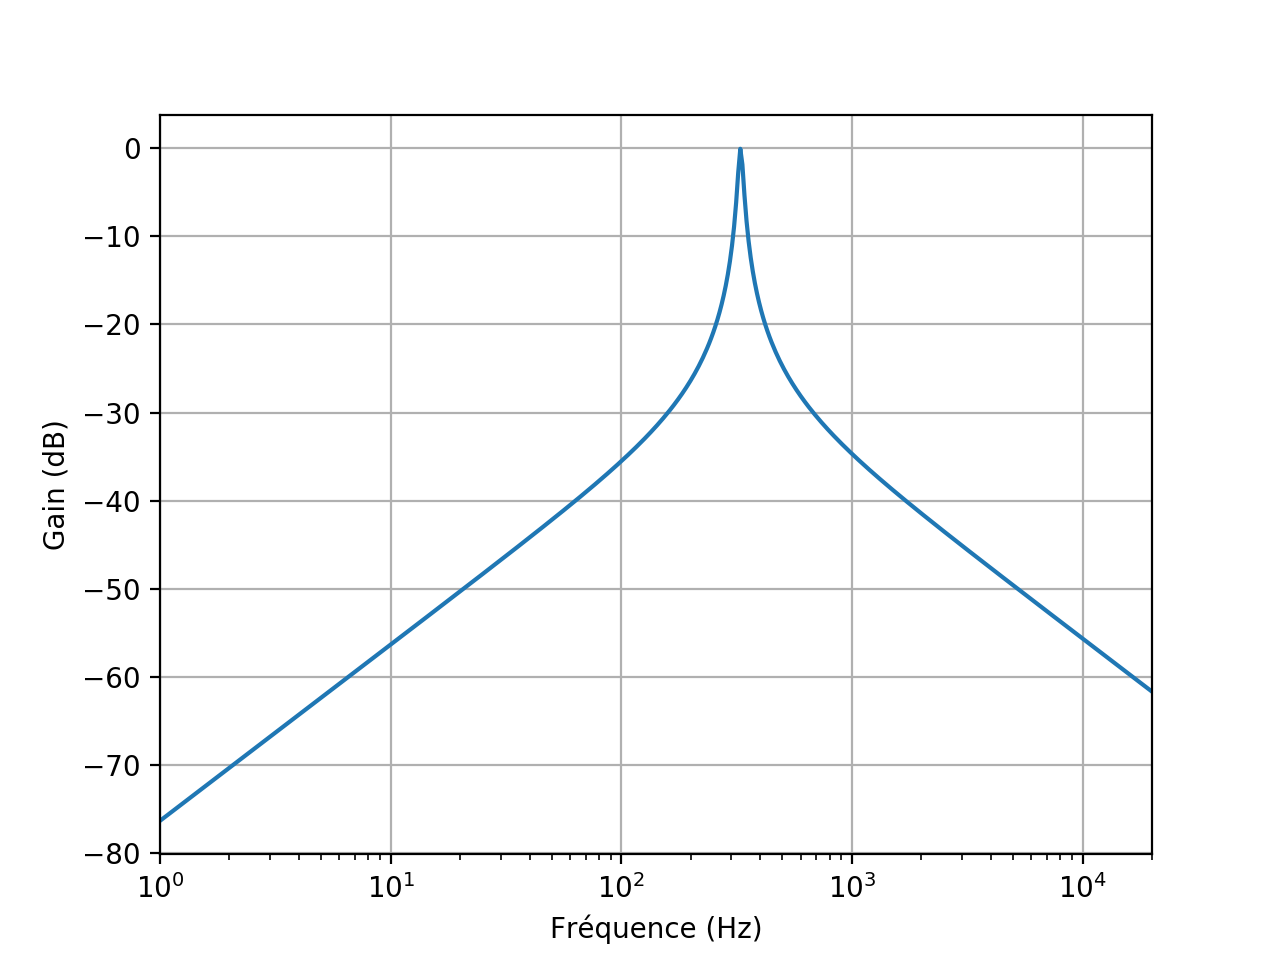
\includegraphics[width=0.9\linewidth]{dm6fig/Fig-passebande-bode-2}
	\end{minipage}
	%
	\begin{minipage}[c]{0.49\linewidth}
		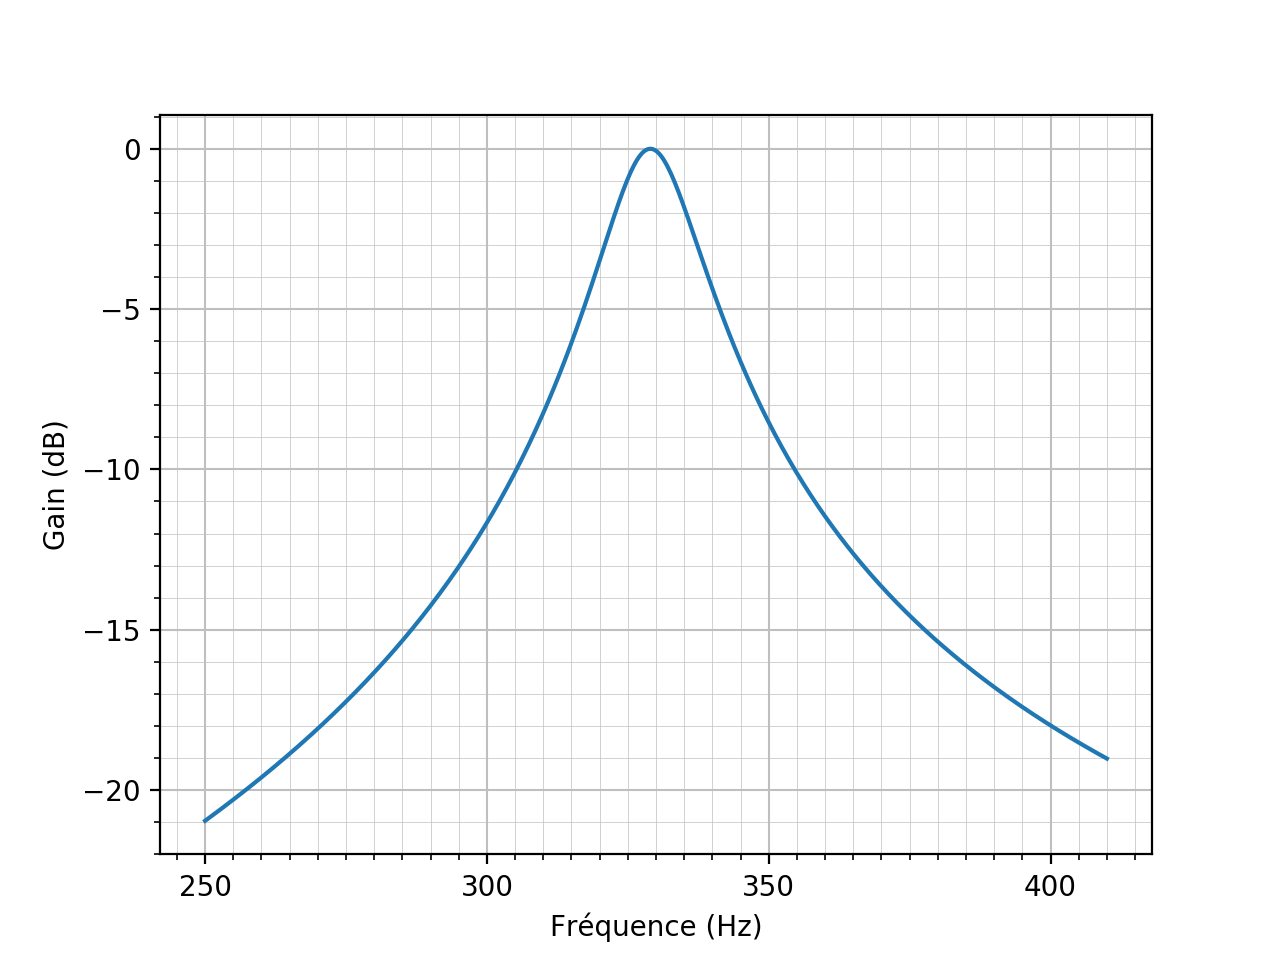
\includegraphics[width=0.9\linewidth]{dm6fig/Fig-passebande-bode-1}
	\end{minipage}
\end{center}


\begin{enumerate}[resume]
	\item Dire en le justifiant rapidement, de quel type de filtre il s'agit. Quelle est sa fréquence centrale caractéristique ?
	
	\boxans{
	    La forme croissante puis décroissante du diagramme indique un \boxsol{filtre passe-bande}. L'abscisse du maximum indique alors la fréquence caractéristique, qu'on détermine ici comme valant \boxsol{$\SI{330}{\hertz}$}.
	}
	
	\item Donner une estimation de sa bande-passante après l'avoir définie.
	
	\boxans{
	    Avec $G_\text{max}$ le gain maximum la bande-passante est alors définie comme l'ensemble des fréquences $f$ telles que le gain vérifie $G(f) \leq \dfrac{G_\text{max}}{\sqrt{2}}$, soit, par croissance de $\log$, $G_\text{dB}(f) \leq G_\text{dB}\left(G_\text{max}\right) - 10\log(2)$. On repère graphiquement que le gain en décibels maximum vaut $G_\text{dB}\left(G_\text{max}\right) = G_\text{dB,max} = \SI{0}{\dB}$. On défini donc la bande passante comme\boxsol{l'ensemble des fréquences $f$ vérifiant $G_\text{dB}(f) \geq \SI{-3}{\dB}$}. Graphiquement, on trouve \boxsol{$f \in \left[\SI{320}{\hertz}, \SI{340}{\hertz}\right]$}.
	}
	
	\item Si la corde est désaccordée à $f_\text{co} = \SI{315}{\hertz}$, estimer, en le justifiant, de quel facteur est atténuée sa composante spectrale fondamentale en sortie de ce filtre.
	
	\boxans{
	    On repère graphiquement que le gain en décibels pour la fréquence $f_\text{co}$ vaut environ $G_\text{dB}\left(f_\text{co}\right) \approx \SI{-6}{\dB}$. Or $G_\text{dB}\left(f_\text{co}\right) = 20\log{G\left(f_\text{co}\right)}$, donc \boxsol{$G\left(f_\text{co}\right) = 10^{\frac{1}{20}G_\text{dB}\left(f_\text{co}\right)}$}. L'application numérique donne \boxsol{$G\left(f_\text{co}\right) \approx 0,5$}. La composante spectrale fondamentale du signal sera donc divisée par un facteur 2 lors de son passage dans le filtre.
	    
	    En considérant la succession des filtres, on peut en fait calculer le gain total sur cette composante : $G_\text{total} = G_1\left(f_\text{co}\right)\times\mod{\underline H_2\left(f_\text{co}\right)}\times G_3\left(f_\text{co}\right)$. Donc :
	    
	    \[\boxsol{$G_\text{total} = \dfrac{2R_1C_1\pi f_\text{co}}{\sqrt{1 + \left(2R_1C_1\pi f_\text{co}\right)^2}}\times \dfrac{\sqrt{\left(1+\frac{R_2}{R_3}\right)^2 + \left(2R_2C_2\pi f_\text{co}\right)^2}}{\sqrt{1+\left(2R_2C_2\pi f_\text{co}\right)^2}} \times 10^{\frac{1}{20}G_\text{dB}\left(f_\text{co}\right)}$}\]
	    
	    L'application numérique donne \boxsol{$G_\text{total} \approx 48$}. En sortie des trois filtres, la composante fondamentale du signal a donc été multiplie par 48.
	}
\end{enumerate}


\subsection{Analyse spectrale}

La figure \ref{spectre1} correspond au spectre en amplitude du signal d'entrée
$u_\text{e}$ représenté sur la figure \ref{signal}.

\begin{center}
	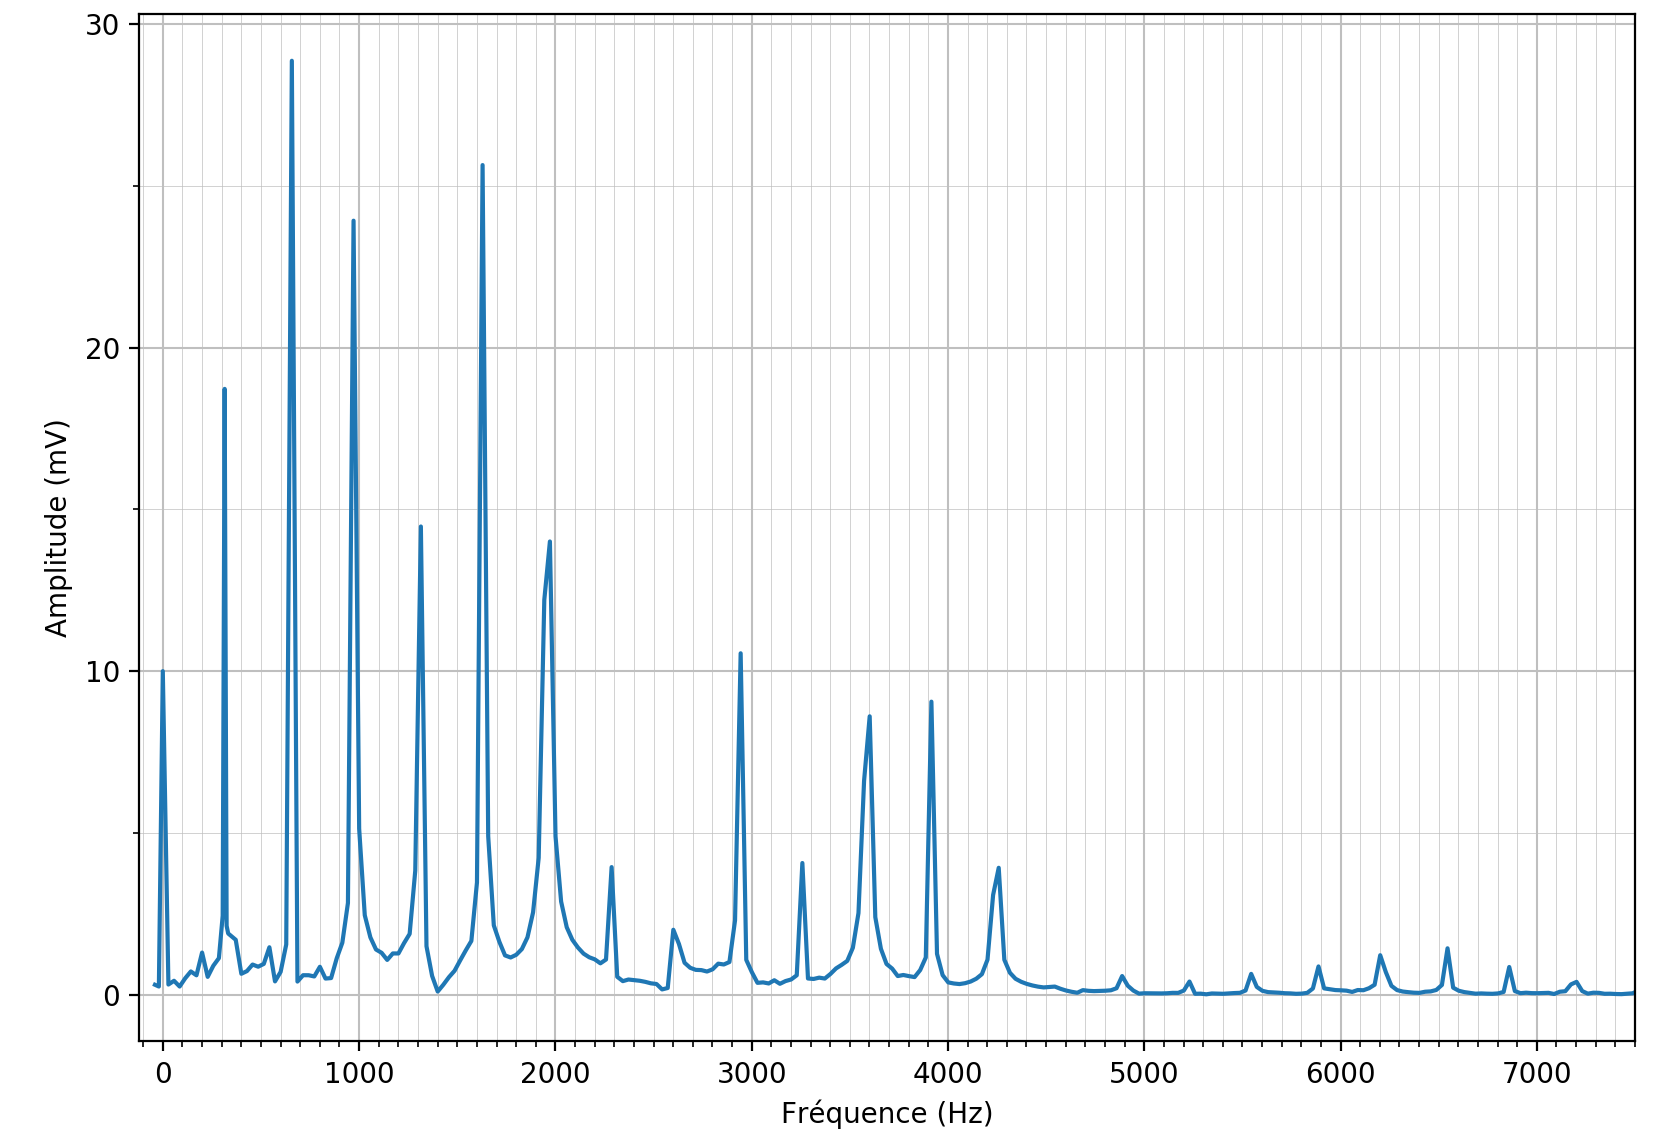
\includegraphics[scale=0.48]{dm6fig/Fig-spectre1.png}
	\captionof{figure}{Spectre en amplitude du signal d’entrée.}
	\label{spectre1}
\end{center}

\begin{enumerate}[resume]
	\item Justifier qu'il est parfaitement cohérent qu'il s'agisse du spectre du signal de la figure \ref{signal}.
	
	\boxans{
	    On remarque que les \guill{pics} d'amplitude du spectre surviennent tous les \SI{300}{\hertz} environ, ce qui correspond bien aux harmoniques/multiples de la fréquence fondamentale $f_\text{co}$ figure \ref{signal}, établie en question \enumref{qu:3}. On remarque également que l'intensité de l'harmonique de fréquence nulle correspond bien à la valeur de $\phyavg{u_e}$ déterminée à la question \enumref{qu:1}. \boxsol{Il s'agit donc bien du spectre du signal de la figure \ref{signal}}.
	}

	\item En le justifiant soigneusement, dire quel spectre de la figure \ref{spectre2} correspond à la sortie du premier filtre $F_\text{a}$.
	
	\boxans{
	    Le premier filtre $F_\text{a}$ va grandement réduire l'intensité de la portion du signal pour les fréquences inférieures à $f_1 \approx \SI{16}{\hertz}$. Le pic observée vers $\SI{0}{\hertz}$ sera donc éliminé, ce qui élimine la réponse (C). Similairement, le filtre que très peu affecter le signal pour les autres fréquences, ainsi on doit toujours pouvoir observer les pics entre $\SI{5000}{\hertz}$ et $\SI{8000}{\hertz}$, ce qui élimine la réponse (D). Enfin, la filtre n'a aucun effet amplificateur, son gain maximum valant $1$. On peut donc éliminer la réponse (B). Il s'agit donc de la \boxsol{réponse (A)}.
	}

	\item Même question pour la sortie du filtre $F_\text{b}$.
	
	\boxans{
	    Le pic vers $\SI{0}{\hertz}$ a été éliminé par le premier filtre\footnote{Si l'on considère que le signal ne passe pas préalablement par le filtre $F_\text{a}$, alors il s'agit plutôt de la \boxsol{réponse (C)}} et ne peut pas revenir, ce qui élimine d'office la réponse (C). Le gain minimum du deuxième filtre est par ailleurs $1$, le filtre ne peut donc pas absorber les pics entre $\SI{5000}{\hertz}$ et $\SI{8000}{\hertz}$, ce qui élimine la réponse (D). Enfin, l'aspect fortement amplificateur élimine la réponse (A). Il s'agit donc de la \boxsol{réponse (B)}. 
	}

	\item Tracer l'allure du spectre en amplitude du signal en sortie du filtre
	$F_\text{c}$. Tracer l'allure du signal (temporel) correspondant.
	
	\boxans{
	    Tracer le spectre en sortie du filtre $F_\text{c}$ revient à considérer pour chaque fréquence $f$ l'amplitude $A_{(B)}(f)$ sur le spectre (B) et le gain en décibels $G_\text{dB}(f)$ sur le diagramme de Bode plus-haut, mesurer graphiquement ces valeurs, puis tracer $A_{(C)}$, où :
	    \[ A_{(C)}(f) = A_{(B)}(f) \times 10^{-\frac{1}{20}G_\text{dB}(f)}\]
	    
	    Concrètement, on ne va considérer que les \guill{pics} du spectre (B), l'essentiel de l'information étant contenu dans ces derniers. On obtient donc $n = 22$ fréquences $f_\text{k} = kf_\text{co}$ pour ces pics. Le signal temporel correspondant vaut alors :
	    \[ s_3(t) = c + \sum_{k = 1}^n A_{(C)}(f_\text{k})\cos{2\pi f_\text{k}t} = \sum_{k = 1}^n A_{(C)}(kf_\text{co})\cos{2k\pi f_\text{co}t}\]
	    
	    où $c$ correspond à l'amplitude de \guill{l'harmonique de fréquence nulle}. Celle-ci ayant été filtrée par $F_\text{a}$, on considérera donc $c = \SI{0}{\mV}$.\\[-5pt]
	    
	    Il aurait fallu, pour plus de précision, disposer d'un spectre en phase pour les différentes harmoniques, ces dernières étant ici (signal en bleu ci-dessous) pas toutes en phase, comme montré par la formule ci-dessus. Ceci semble assez improbable puisque ces fréquences sont d'une part déphasés dans le signal d'origine, et d'autre part que les différents filtres ont un comportement déphasant. Ces déphasages peuvent avoir un effet conséquent sur l'allure du signal, comme montré dans l'exemple du signal en violet ci-dessous, où la fondamentale est déphasée de $0.9$ radians et la première harmonique de $4.9$ radians.\\[-5pt]
	    
	    On obtient donc finalement le spectre en amplitude et les signaux temporels ci-dessous :
	    
	    \begin{center}
            \boxsol{
            \begin{minipage}[c]{0.48\linewidth}
            \pgfplotsset{width=10cm}
            \begin{tikzpicture}[scale = 0.7]
                \begin{axis}[
                    axis lines = left,
                    xlabel=$\textsf{Fréquence (Hz)}$,
                    ylabel=$\textsf{Amplitude (mV)}$,
                    xmin=0,
                    xmax=8000,
                    ymin=0,
                    ymax=250,
                    xtick distance={1000},
                    ytick distance={100},
                    xticklabel={$\mathsf{\pgfmathprintnumber{\tick}}$},
                    yticklabel={$\mathsf{\pgfmathprintnumber{\tick}}$},
                    minor x tick num=9,
                    minor y tick num=3,
                    x tick label style={/pgf/number format/1000 sep=\,},
                    font=\footnotesize,
                    grid = both,
                    grid style = {line width = .1pt, draw = gray!30},
                    major grid style = {line width=.2pt,draw=gray!50},
                ]
                    \addplot[mark=none, main1, line width=0.6mm] coordinates {(315,0) (315,225)};
                    
                    \addplot[mark=none, main1, line width=0.6mm] coordinates {(630,0) (630,27)};
                    
                    \addplot[mark=none, main1, line width=0.6mm] coordinates {(945,0) (945,9.8)};
                    
                    \addplot[mark=none, main1, line width=0.6mm] coordinates {(1260,0) (1260,3.5)};
                    
                    \addplot[mark=none, main1, line width=0.6mm] coordinates {(1575,0) (1575,4.76)};
                    
                    \addplot[mark=none, main1, line width=0.6mm] coordinates {(1890,0) (1890,1.9)};
                    
                    \addplot[mark=none, main1, line width=0.6mm] coordinates {(2205,0) (2205,0.5)};
                    
                    \addplot[mark=none, main1, line width=0.6mm] coordinates {(2520,0) (2520,0.2)};
                    
                    \addplot[mark=none, main1, line width=0.6mm] coordinates {(2835,0) (2835,1.3)};
                    
                    \addplot[mark=none, main1, line width=0.6mm] coordinates {(3150,0) (3150,0.4)};
                    
                    \addplot[mark=none, main1, line width=0.6mm] coordinates {(3465,0) (3465,1.1)};
                    
                    \addplot[mark=none, main1, line width=0.6mm] coordinates {(3780,0) (3780,1.1)};
                    
                    \addplot[mark=none, main1, line width=0.6mm] coordinates {(4095,0) (4095,0.3)};
                    
                    \addplot[mark=none, main1, line width=0.6mm] coordinates {(4410,0) (4410,0.05)};
                    
                    \addplot[mark=none, main1, line width=0.6mm] coordinates {(4725,0) (4725,0.1)};
                    
                    \addplot[mark=none, main1, line width=0.6mm] coordinates {(315*16,0) (315*16,0.1)};
                    
                    \addplot[mark=none, main1, line width=0.6mm] coordinates {(315*17,0) (315*17,0.1)};
                    
                    \addplot[mark=none, main1, line width=0.6mm] coordinates {(315*18,0) (315*18,0.1)};
                    
                    \addplot[mark=none, main1, line width=0.6mm] coordinates {(315*19,0) (315*19,0.1)};
                    
                    \addplot[mark=none, main1, line width=0.6mm] coordinates {(315*20,0) (315*20,0.1)};
                    
                    \addplot[mark=none, main1, line width=0.6mm] coordinates {(315*21,0) (315*21,0.1)};
                    
                    \addplot[mark=none, main1, line width=0.6mm] coordinates {(315*22,0) (315*22,0.1)};
                \end{axis}
            \end{tikzpicture}
            \end{minipage}
            %
	        \hfill
	        %
            \begin{minipage}[c]{0.48\linewidth}
            \pgfplotsset{width=10cm}
            \begin{tikzpicture}[scale = 0.7]
                \begin{axis}[
                    axis lines = left,
                    xlabel=$\textsf{Temps (ms)}$,
                    ylabel=$\textsf{Signal (mV)}$,
                    xmin=0,
                    xmax=10,
                    ymin=-300,
                    ymax=300,
                    xtick distance={1},
                    ytick distance={100},
                    xticklabel={$\mathsf{\pgfmathprintnumber{\tick}}$},
                    yticklabel={$\mathsf{\pgfmathprintnumber{\tick}}$},
                    minor x tick num=4,
                    minor y tick num=4,
                    x tick label style={/pgf/number format/1000 sep=\,},
                    font=\footnotesize,
                    grid = both,
                    grid style = {line width = .1pt, draw = gray!30},
                    major grid style = {line width=.2pt,draw=gray!50},
                    trig format plots=rad,
                ]
                    \addplot[color=main1, line width=0.6mm, domain=0:10,  smooth,samples=200] {225*cos(1.98*x)+27*cos(3.96*x)+9.8*cos(5.94*x)+3.5*cos(7.9*x)+4.76*cos(9.9*x)+1.9*cos(12*x)+0.5*cos(14*x)+0.2*cos(16*x)+1.3*cos(18*x)+0.4*cos(20*x)+1.1*cos(22*x)+1.1*cos(24*x)};
                    
                    \addplot[color=main3, line width=0.4mm, domain=0:10,  smooth,samples=200] {225*cos(1.98*x+0.9)+27*cos(3.96*x+4.9)+9.8*cos(5.94*x)+3.5*cos(7.9*x)+4.76*cos(9.9*x)+1.9*cos(12*x)+0.5*cos(14*x)+0.2*cos(16*x)+1.3*cos(18*x)+0.4*cos(20*x)+1.1*cos(22*x)+1.1*cos(24*x)};
                \end{axis}
            \end{tikzpicture}
            \end{minipage}
            }
        \end{center}
	}
\end{enumerate}

\medskip

\begin{center}
	\begin{minipage}[c]{0.48\linewidth}
		\centering
		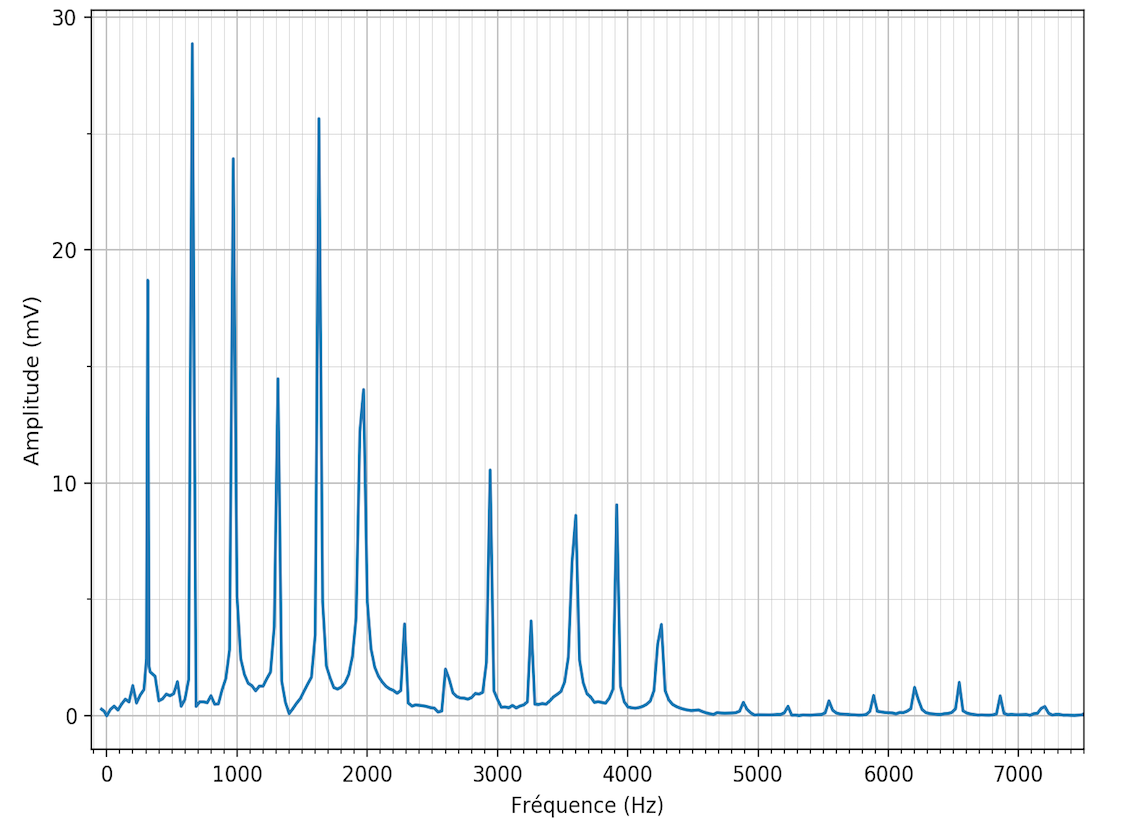
\includegraphics[width=0.98\linewidth]{dm6fig/Fig-spectre2.png}\\
		(A)
	\end{minipage}
	%
	\hfill
	%
	\begin{minipage}[c]{0.48\linewidth}
		\centering
		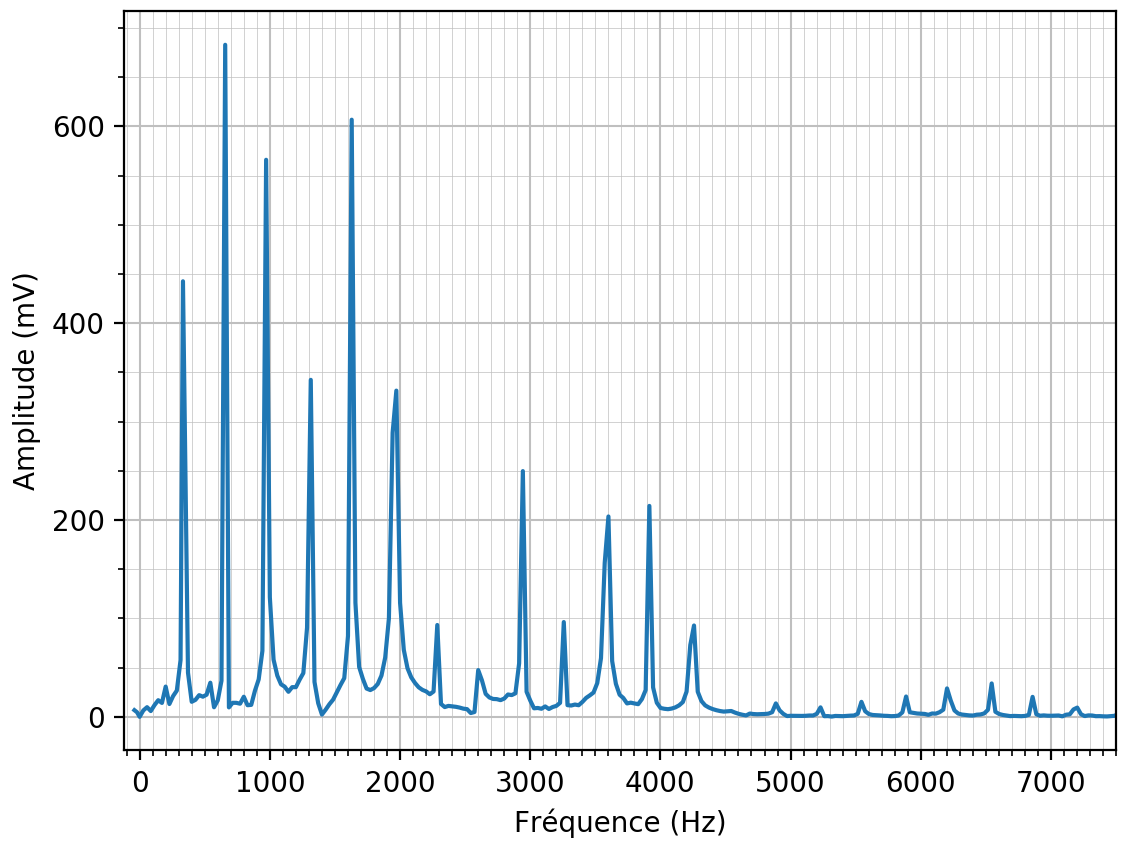
\includegraphics[width=0.98\linewidth]{dm6fig/Fig-spectre6.png}\\
		(B)
	\end{minipage}
	
	\medskip

	\begin{minipage}[c]{0.48\linewidth}
		\centering
		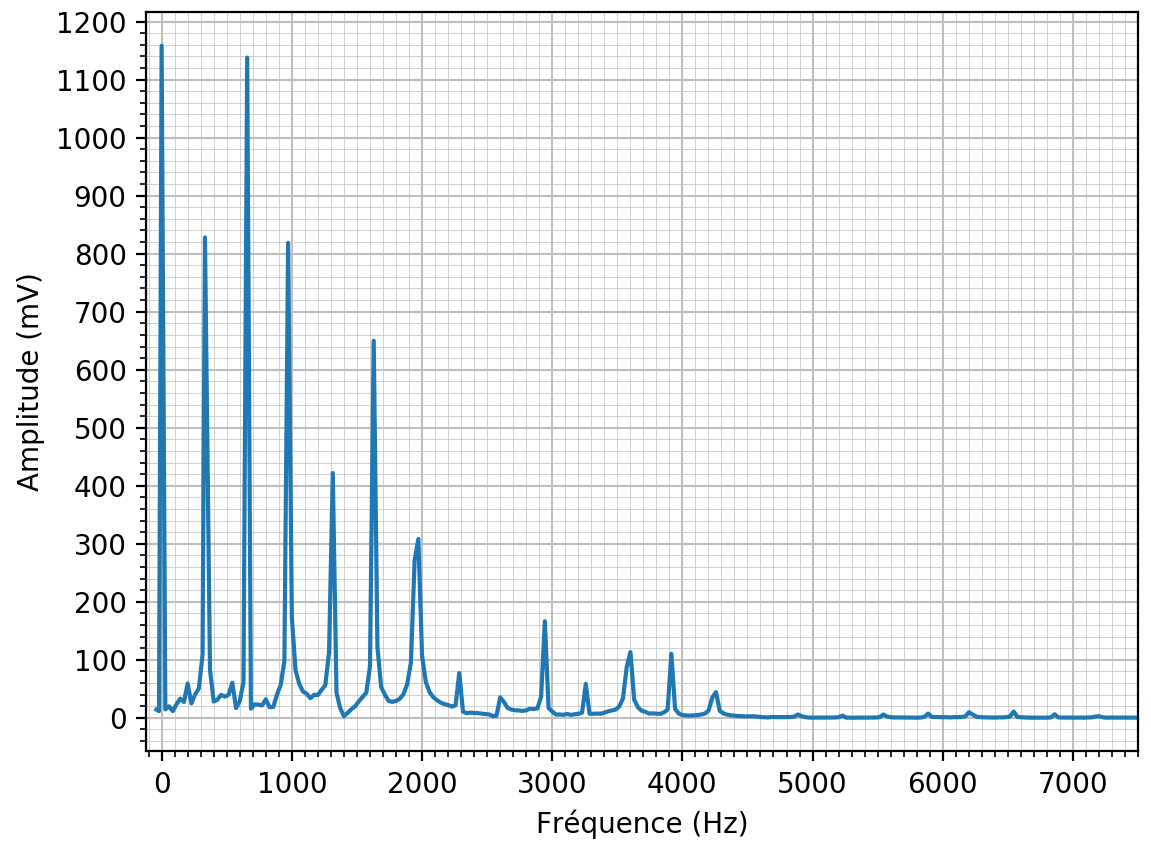
\includegraphics[width=0.98\linewidth]{dm6fig/Fig-spectre5.png}\\
		(C)
	\end{minipage}
	%
	\hfill
	%
	\begin{minipage}[c]{0.48\linewidth}
		\centering
		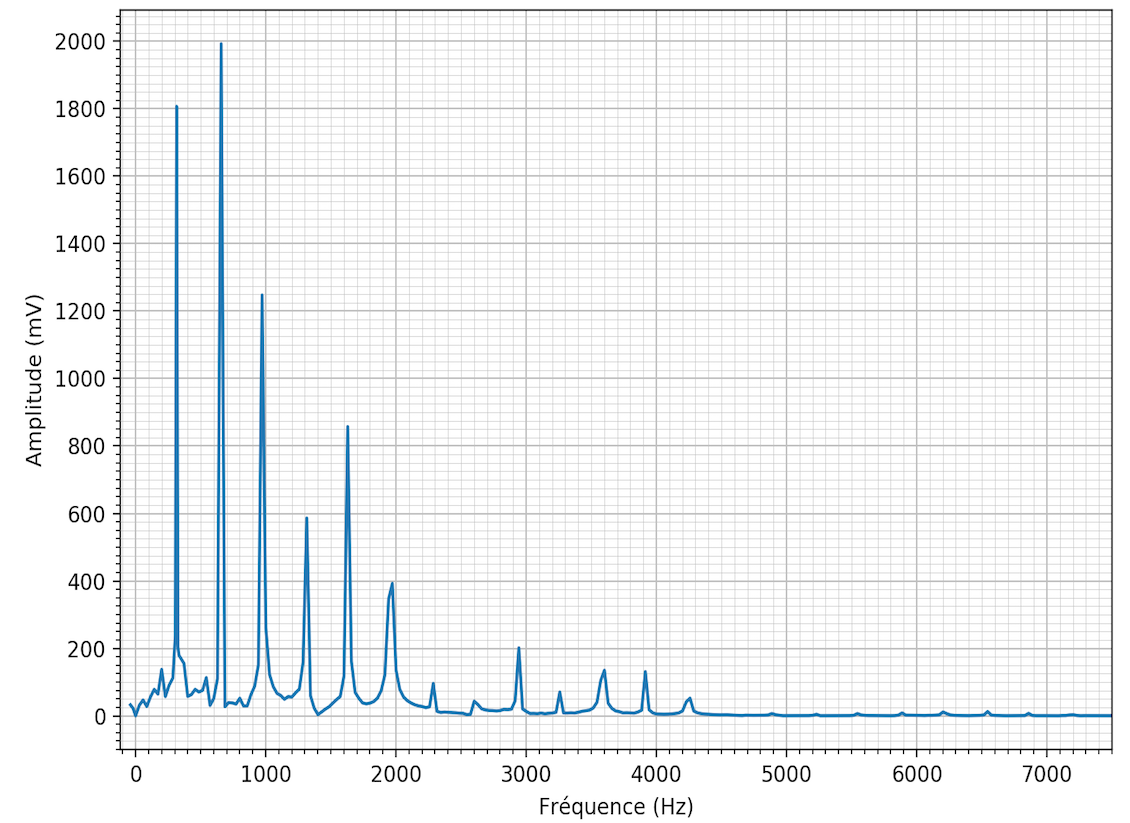
\includegraphics[width=0.98\linewidth]{dm6fig/Fig-spectre3.png}\\
		(D)
	\end{minipage}
	
	\captionof{figure}{Spectres en amplitude possibles.}
	\label{spectre2}
\end{center}

\end{document}

